\chapter{PID com servovisão por posição (PBVS)}
\label{cap:pid}

\section{Lei de controle}
Arquivo \code{control/pbvs\_pid\_controller.cpp}. O erro é o ponto de perseguição
$\vect e = \vect p_{des} = \rr - d\rhat$ (sinal contrário de $\ep$), e a saída é uma
\textbf{velocidade}:
\begin{equation}
  \vect v_{cmd} = k_{ff}\,\vect v_t + k_p\,\vect e + k_i\!\int\!\vect e\,dt + k_d\,\dot{\vect e},
  \qquad
  \dot{\vect e} = \dot\rr - \frac{d}{\lVert\rr\rVert}\left(\vect I-\rhat\rhat\T\right)\dot\rr .
  \label{eq:pid}
\end{equation}
A derivada é \emph{analítica}: usa a velocidade relativa do KF, sem derivar a medida
ruidosa. O integrador só acumula quando $\lVert\vect e\rVert<$ \code{integral\_zone}
(integração condicional) e tem a norma de $k_i\!\int\!\vect e$ limitada a
\code{integral\_limit} (anti-windup). Valores do \code{yaml}: $k_p=0{,}8$, $k_i=0{,}05$,
$k_d=0{,}2$, $k_{ff}=1$.

\section{Dinâmica do erro com seguimento ideal}
Suponha que a PX4 siga a velocidade perfeitamente ($\vect v_c=\vect v_{cmd}$) e despreze
a rotação da LOS. Então $\dot e = v_t - v_c$ e, com $k_{ff}=1$:
\begin{equation}
  \dot e = -k_p e - k_i\!\int\! e - k_d\dot e
  \;\Longrightarrow\;
  (1+k_d)\,s^2 + k_p\,s + k_i = 0 .
  \label{eq:pid-car}
\end{equation}
O termo derivativo funciona como uma ``massa'' que \emph{reduz} o ganho efetivo:
\begin{equation}
  \omega_n = \sqrt{\frac{k_i}{1+k_d}},\qquad
  2\zeta\omega_n = \frac{k_p}{1+k_d}.
\end{equation}
Com o \code{yaml}: $1{,}2s^2+0{,}8s+0{,}05=0\Rightarrow s=-0{,}60$ e $s=-0{,}07$. O polo
rápido dá a constante de tempo de aproximação
$\tau_e=(1+k_d)/k_p=\SI{1,5}{s}$. O polo lento (\SI{14}{s}) é o do integrador, que só
corrige viés residual.

\paragraph{Papel do feedforward.} Sem $k_{ff}$, um alvo a velocidade constante produz o
erro estacionário $e_{ss}=v_t/k_p$ (para $v_t=\SI{1,5}{m/s}$ e $k_p=0{,}8$: \SI{1,9}{m}!).
O integrador zeraria esse erro, mas lentamente. Com $k_{ff}=1$ o erro de regime é nulo
mesmo sem $k_i$, desde que $\vect v_t$ esteja bem estimada.

\section{Cálculo dos ganhos}
\subsection{Por alocação de polos (modelo ideal)}
Sem integrador, \eqref{eq:pid-car} vira $(1+k_d)s+k_p=0$, de 1ª ordem. Escolha a
constante de tempo $\tau_e$ e a razão $k_d$:
\begin{equation}
  k_p = \frac{1+k_d}{\tau_e}.
\end{equation}
Com integrador, imponha $\omega_n,\zeta$ e resolva
$k_i = (1+k_d)\omega_n^2$ e $k_p = 2\zeta\omega_n(1+k_d)$. Exemplo: $\tau_e=\SI{0,8}{s}$
($\omega_n=1{,}25$, $\zeta=1$) e $k_d=0{,}2$ dão $k_p=3{,}0$ e $k_i=1{,}9$. Esse
integrador é agressivo; prefira $\omega_n$ do integrador 3--5 vezes menor que o polo
proporcional.

\subsection{Pelo lugar das raízes com a PX4 e o atraso}
Com a malha interna \eqref{eq:tv} e o atraso, a malha aberta é
\begin{equation}
  L(s) = \left(k_p + \frac{k_i}{s} + k_d s\right)\frac{T_v(s)}{s}\,e^{-s\tau}.
\end{equation}
Fixe as razões $k_d/k_p$ e $k_i/k_p$ (posição dos zeros) e trace o LGR em $k_p$. No
discreto, use $P(z) = \text{c2d}(T_v/s,\Ts,\text{zoh})\cdot z^{-2}$ e o PID discreto
$C(z)=k_p + k_i\Ts\frac{z}{z-1} + k_d\frac{z-1}{\Ts z}$.

\begin{figure}[H]
\centering
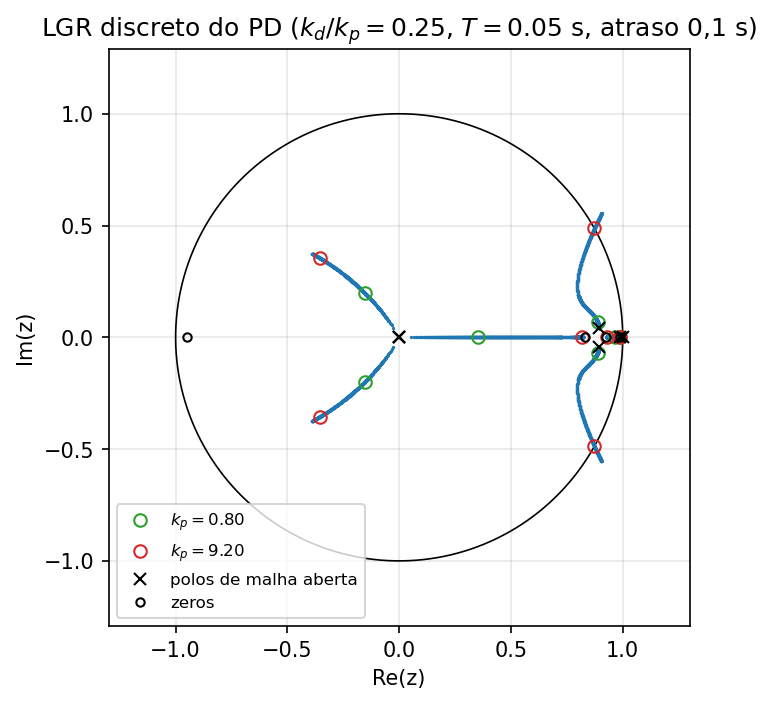
\includegraphics[width=0.55\textwidth]{lgr_pid_discreto.png}
\caption{LGR discreto do PD ($k_d/k_p=0{,}25$) com a PX4 e \SI{0,1}{s} de atraso. Em
$k_p=0{,}8$ (verde) os polos dominantes estão bem dentro do círculo. A instabilidade
ocorre em $k_p\approx9{,}2$ (vermelho): o \emph{ganho crítico} $K_u$.}
\label{fig:lgr-pid}
\end{figure}

\begin{receita}
\textbf{PID pelo LGR (\code{matlab/projeto\_pid.m}).}
\begin{enumerate}
  \item Monte $P(z)$ com \code{modelo\_px4.m} e o atraso de \code{parametros.m}.
  \item Escolha os zeros: $k_d/k_p\in[0{,}1;0{,}3]$ e $k_i/k_p\in[0{,}02;0{,}1]$.
  \item \code{rlocus(C0*P)} com \code{zgrid(zeta, wn*Ts)}. Escolha $k_p$ no cruzamento
        do ramo dominante com $\zeta=0{,}7$.
  \item Confira com \code{margin}: PM $\ge\ang{45}$ e margem de ganho $\ge\SI{6}{dB}$
        ($K_u/k_p\ge2$).
  \item Simule com saturação e ruído (\code{sim\_perseguicao.m}).
\end{enumerate}
\end{receita}

\subsection{Ziegler--Nichols (ponto de partida)}
Do LGR (ou de um ensaio no Gazebo aumentando $k_p$ até oscilar) obtém-se $K_u$ e o
período de oscilação $P_u$. A tabela clássica ($k_p=0{,}6K_u$, $T_i=P_u/2$,
$T_d=P_u/8$) foi feita para plantas sem integrador e dá ganhos agressivos aqui. Use-a
só como limite superior e reduza $k_p$ até atingir a margem desejada.

\section{PID ótimo}
\subsection{Equivalência com LQR (modelo ideal)}
Com seguimento ideal, a planta de um eixo é um integrador simples, $\dot e = -v_c + v_t$.
O LQR com estado aumentado $z=[\int e,\ e]$ e custo
$\int(q_i\xi^2 + q_p e^2 + r v^2)dt$ produz exatamente um PI:
$v = k_p e + k_i\int e$. Assim, $k_p,k_i$ saem de \code{lqr} sobre
$A=\begin{bsmallmatrix}0&1\\0&0\end{bsmallmatrix}$, $B=\begin{bsmallmatrix}0\\-1\end{bsmallmatrix}$
(ver \code{projeto\_pid.m}, seção ``PID ótimo LQ'').

\subsection{Otimização numérica (recomendada para a comparação)}
Defina $\theta=[k_p,k_i,k_d]$ e minimize um custo simulado da malha \emph{completa}
(PX4 + atraso + ruído + saturação), por exemplo
\begin{equation}
  J(\theta) = \frac1{T}\int_0^T\!\left(\lVert\vect e\rVert^2 + \rho\lVert\vect a_c\rVert^2\right)dt
  + \mu\,\max(0,\ \ang{45}-\text{PM}(\theta))^2 ,
\end{equation}
com \code{fminsearch} a partir dos ganhos do LGR. O termo de margem impede que o
otimizador escolha ganhos frágeis que só funcionam no cenário de treino.
Implementado em \code{otimizar\_ganhos.m}.

\section{Implementação discreta}
O código implementa \eqref{eq:pid} com integração de Euler
($\xi_{k+1}=\xi_k+\Ts e_k$) e derivada analítica. Como a saída é velocidade, a
aceleração enviada à PX4 é $(\vect v_{cmd}-\vect v_{ref})/\Ts$, limitada por
\code{max\_acc}. Esse feedforward por diferença finita é ruidoso e é a principal
diferença prática em relação aos controladores de aceleração.
